%===============================
%------------------------------
\section{Postulates of quantum theory}
%------------------------------
%===============================

%---------------------------------------------
\subsection{Quantum states and basis measurements}
%---------------------------------------------

\begin{empheq}[box=\fbox]{align}
	\textrm{State} &\longleftrightarrow \textrm{Vector}  \\
	\textrm{Measurement} &\longleftrightarrow \textrm{Projection operator} \\
	\textrm{Dynamics} &\longleftrightarrow \textrm{Unitary operator}  
\end{empheq}


Any ONB gives a {\bf basis measurement}, which defines a probability distribution,
\begin{align}
	p_k &= \abs{\av{e_k|\psi}}^2 = \langle\psi {\color{teal}\overbracket{\dyad{e_k}}^{\op P_k}} \psi \rangle = \expval{\op P_k}{\psi},
\end{align}
$\sum_k \op P_k = \op\id$. For $p_k$ to be a probability, the state must therefore be normalized to 1:
\begin{align}
	\norm{\psi} = \sqrt{\av{\psi|\psi}} = 1.
\end{align}
After the measurement, the state is updated to the basis state $\ket{e_k}$ through the action of the projector,
\begin{align}
	\frac{\op P_k\ket{\psi}}{\sqrt{p_k}} = \frac{\op P_k\ket{\psi}}{\sqrt{\expval{\op P_k}{\psi}}}.
\end{align}
Observe that multiplying a state vector by a complex phase has no effect on any empirical prediction. This can be seen from the following equation.
\begin{align}
	|\mel{\phi}{e^{i\delta}}{\psi}|^2 &= \cancelto{1}{|e^{i\delta}|^2} \abs{\av{\phi|\psi}}^2
\end{align}
This type of phase is commonly referred to as a {\bf global phase} as opposed to a {\bf relative phase}, which, on the other hand, gives rise to interference phenomena, a hallmark of quantum theory.
\begin{align}
	\abs{\bra{\phi}(\ket{\psi_1} + e^{i\delta} \ket{\psi_2})}^2 &= |{\color{maincolor}\overbracket{\color{black}\av{\phi|\psi_1}}^{\psi_1}} + e^{i\delta}{\color{eqcolor}\overbracket{\color{black}\av{\phi|\psi_2}}^{\psi_2}}|^2 \\
	&= \abs{\psi_1}^2 + \abs{\psi_2}^2 + {\color{magenta}\underbracket{2\mathrm{Re}(e^{i\delta}\psi_1^* \psi_2)}_{\textrm{Quantum interference}}}
\end{align}



%---------------------------------------------
\subsection{Case study: qubit}
%---------------------------------------------

A two-level system, or a \emph{qubit}, is any quantum system that can be described by a two-dimensional Hilbert space. We denote the standard ONB as $\{\ket{0},\ket{1}\}$.
\begin{align}
	\ket{\psi} &= \alpha\ket{0} + \beta\ket{1} \\
	&=  ae^{i\gamma}\ket{0} + be^{i\delta}\ket{1} \mnf{Polar form where $a,b,\gamma,\delta$ are real numbers.} \\
	&=e^{i\gamma}\biggl[{\color{maincolor}\underbrace{\cos(\frac{\theta}{2})}_{a}} \ket{0} + e^{i{\color{teal}\tikzmark{a}\varphi}} {\color{eqcolor}\underbrace{\sin(\frac{\theta}{2})}_{b}}\ket{1}\biggr]
\end{align}
\begin{tikzpicture}[remember picture,overlay]
	\draw[<-] 
	([shift={(3pt,6pt)}]a) |- ([shift={(10pt,20pt)}]a) 
	node[anchor=west] {\scriptsize{\color{teal}$\delta-\gamma$}}; 
\end{tikzpicture}
By normalizing the state vector and eliminating the global phase, we have parametrized the state of a qubit by two spherical coordinate $0\le \theta \le \pi$ and $0\le \varphi < 2\pi$.
\begin{figure}[h]
	\centering
	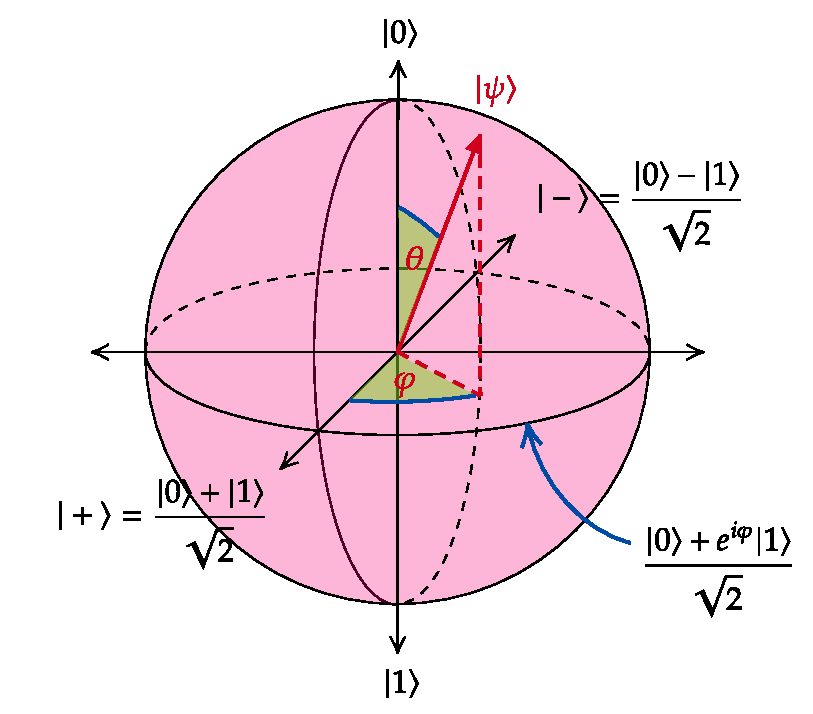
\includegraphics[scale=0.75]{fig/bloch.pdf}
	\caption{Space of qubit states is represented by the Bloch sphere.}
	\label{}
\end{figure}

\noindent Why the one half in $\theta/2$? Look at the operator space,\mn{Given a general state of a two-level system, $\ket{\psi}=\alpha\ket{0}+\beta\ket{1}$, the orthogonal state (up to a phase) can be written as $\ket{\psi^{\perp}}=-\beta^*\ket{0}+\alpha^*\ket{1}$.}
\begin{align}
	\ket{\bf \hat n} &= \cos(\theta/2) \ket{0} + \sin(\theta/2) e^{i\varphi} \ket{1} \\
	\ket{\bf -\hat n} &= -\sin(\theta/2)e^{-i\varphi} \ket{0} + \cos(\theta/2) \ket{1}
\end{align}
\begin{align}
	\dyad{\bf \hat n} &\longleftrightarrow \frac{1}{2} \mqty(1+\cos\theta && \sin\theta\,e^{-i\varphi} \\ \sin\theta\,e^{i\varphi} && 1-\cos\theta)  \mnf{Angel doubling formulae: 
	\begin{align*}
	\sin(\theta) &= 2\sin(\theta/2)\cos(\theta/2), \\
	\cos(\theta) &= \cos^2(\theta/2) - \sin^2(\theta/2) \\ 
	&= 2\cos^2(\theta/2) - 1.	
	\end{align*}} \\
	&= \frac{1}{2}\mqty(1+z & x-iy \\ x+iy & 1-z) \\
	&= \boxed{\frac{\id + \boldsymbol{\hat n \cdot \sigma}}{2}}\, , 
\end{align}
where 
\begin{align}
	\boldsymbol{\sigma} = \mqty(\hat\sigma_x \\ \hat\sigma_y \\ \hat\sigma_z)
\end{align}
is the vector of Pauli matrices
\begin{align}
	\hat\sigma_x = \mqty(0&1\\1&0), &&  \hat\sigma_x = \mqty(0&-i\\i&0), && \hat\sigma_x = \mqty(1&0\\0&-1).
\end{align}
Similarly,\mn{The matrix form can also be obtained from that of $\dyad{\bf \hat n}$ by setting \begin{align*}
		\theta &\leftarrow \pi-\theta, \\
		\varphi &\leftarrow \pi+\varphi. 
\end{align*}}
\begin{align}
	\dyad{\bf -\hat n} &\longleftrightarrow \frac{1}{2} \mqty(1-\cos\theta && -\sin\theta\,e^{-i\varphi} \\ -\sin\theta\,e^{i\varphi} && 1+\cos\theta) = \frac{\id + {(-\boldsymbol{\hat n}) \cdot \boldsymbol\sigma}}{2} 
\end{align}
Spin observable in any direction ${\bf \hat{n}}$
\begin{align}
	\hat\sigma_{\bf \hat n} \equiv \boldsymbol{\hat n\cdot\sigma} = \dyad{\bf \hat n} - \dyad{-\hat {\bf n}} \longleftrightarrow \mqty(\cos\theta && \sin\theta\,e^{-i\varphi} \\ \sin\theta\,e^{i \varphi} && \cos\theta) 
\end{align}
To further investigate the relation between the geometry of the Hilbert space and that of the Euclidean space (inner product $\iff$ geometry), we need to know some properties of Pauli operators.

\vspace{0.5em}
\noindent{\bf Algebraic properties of Pauli operators} 
\begin{enumerate}
	\item $\hat\sigma_j\dgg = \hat\sigma_j$,
	\item $\hat\sigma_j^2 = \id$,
	\item $\hat\sigma_j \hat\sigma_k = i\hat\sigma_l$ where $(j,k,l)$ are cyclic,
	\item $\tr\sigma_j = 0$.
\end{enumerate}
Properties 2 and 3 can be rephrased in terms of the commutator and the anticommutator are
\begin{align}
	[\hat\sigma_j,\hat\sigma_k] = 2i\epsilon_{jkl}\hat\sigma_l, &&
	\{\hat\sigma_j,\hat\sigma_k\} = 2\delta_{jk}\op\id.
\end{align}
Both are encapsulated in the relation
\begin{align}\label{eq:pauli-algebraic}
	\boxed{\hat\sigma_j \hat\sigma_k = \delta_{jk}\op\id + i\epsilon_{jkl}\hat\sigma_l}\, ,
\end{align}
which can be summarized concisely as follows: {\bf Pauli matrices either commute or anticommute}.

\vspace{0.5em}
\noindent 
{\bf Expectation value of Pauli observables.} 
\begin{align}
	\expval{\op\sigma_j}{\bf \hat{n}} &= \tr(\dyad{\bf \hat{n}}\hat\sigma_j) = \tr[\left(\frac{\op\id + \boldsymbol{\hat n \cdot \sigma}}{2}\right)\hat\sigma_j] \\
	&= \frac{1}{2}\tr(\op\sigma_j + \sum_k n_k \hat\sigma_k \hat\sigma_j)
\end{align}
The only term whose trace does not vanish is the identity term from \eqref{eq:pauli-algebraic}. Therefore,
\begin{align}
	\expval{\op\sigma_j}{\bf \hat{n}} &= \frac{1}{2} \sum_k n_k \delta_{jk} \tr \op\id = n_j.
\end{align}
Since a general spin observable is just ${\bf \hat{n}}\cdot \boldsymbol{\sigma}$, the expectation value of spin in $\bf \hat{m}$ direction is ${\bf \hat{n}\cdot\hat{m}}$.
One consequence of this result is that, to determine an unknown state of a two-level system, it is sufficient to find the expectation value of the three Pauli matrices.
\begin{align}
	\mqty(n_x \\ n_y \\ n_z) = \mqty(\av{\hat\sigma_x} \\ \av{\hat\sigma_y} \\ \av{\hat\sigma_z})
\end{align}
This is an example of \emph{quantum state tomography}.

\begin{mybox}[Levi-Civita tensor]
	The Levi-Civita tensor can be used to define the $d$-dimensional totally anti-symmetric vector product. In three dimension,
	\begin{align}
		\epsilon_{jkl} = 
		\begin{cases}
			+1, &(j\;k\;l) \; \textrm{is an \emph{even} permutation} \: (1\; 2\; 3), (2\; 3\; 1), \textrm{or} \; (3\; 1\; 2), \\
			-1, &(j\;k\;l) \; \textrm{is an \emph{odd} permutation} \: (1\; 3\; 2), (2\; 1\; 3), \textrm{or} \; (3\; 2\; 1), \\
			0, &\mathrm{Otherwise}.
		\end{cases}
	\end{align} 
	Here is a few facts about the Levi-Civita tensor. The determinant of a $3\times3$ matrix $M$ can be expressed as the anti-symmetric product of its rows $\det M = \epsilon_{jkl} M_{1j}M_{2k} M_{3l}$. Thus, we have an alternative expression for the cross product:
	\begin{align}
		\vb{A \times B} = \vb{\hat e_j} \epsilon_{jkl} A_k B_l = \det \mqty(\vb{\hat e}_1 & \vb{\hat e}_2 & \vb{\hat e}_3  \\ A_1 & A_2 & A_3 \\ B_1 & B_2 & B_3 ) 
	\end{align}
	A contraction of two Levi-Civita tensors gives an expression involving the Kronecker deltas.
	\begin{align}
		\epsilon_{jkl}\epsilon_{jmn} &= \delta_{km} \delta_{lm} - \delta_{kn} \delta_{lm}, 
		\marginnote{$\delta_{jk}\delta_{jk} = \delta_{jj} = \tr \hat\id_{d\times d} = $ the dimension of the space}\\
		\epsilon_{jkl}\epsilon_{jkm} &= \delta_{kk}\delta_{lm} - \delta_{km} \delta_{lm} = (\dim-1)\delta_{lm} = 2\delta_{lm}
	\end{align}
\end{mybox}

\noindent Now we can compute the inner product in a painless way without needing to use any trigonometric identity.
\begin{align}
	\abs{\ip{\bf \hat n}{\bf \hat m}}^2 &= \frac{1}{4}\tr
	\left[ \left(\id + \boldsymbol{\hat n\cdot\sigma}\right) \left(\id + \boldsymbol{\hat m\cdot\sigma}\right) 
	\right] \\
	&= \frac{1}{4}\tr[ \id +  \underbrace{\boldsymbol{\hat n\cdot\sigma} + \boldsymbol{\hat m\cdot\sigma}}_{\textrm{Traceless}} + (\boldsymbol{\hat n\cdot\sigma})(\boldsymbol{\hat m\cdot\sigma})] \\
	&= \frac{1}{2} + \frac{1}{4}\tr[(\boldsymbol{\hat n\cdot\sigma})(\boldsymbol{\hat m\cdot\sigma})]
\end{align}
What is the trace of $(\boldsymbol{\hat n\cdot\sigma})(\boldsymbol{\hat m\cdot\sigma})$? Use the index notation.
\begin{align}
	(\boldsymbol{\hat n\cdot\sigma})(\boldsymbol{\hat m\cdot\sigma}) &= n_j m_k \hat\sigma_k \hat\sigma_k \\
	&= n_jm_k (\delta_{jk}\id + i\epsilon_{jkl}) \\
	&= n_jm_j\id + i\underbrace{\epsilon_{jkl}n_jm_k}_{({\bf \hat n \times \hat m})_l} \hat\sigma_l \\
	&= ({\bf \hat n \cdot \hat m})\id + \underbrace{({\bf \hat n \times \hat m}) \cdot \boldsymbol{\sigma}}_{\textrm{Traceless}}
\end{align}
To sum up,
\begin{align}
	\boxed{\abs{\ip{\bf \hat n}{\bf \hat m}}^2 = \frac{1+{\bf \hat n \cdot \hat m}}{2}}\, ,
\end{align}  
relating the geometry of the Hilbert space and the Euclidean space. In other words, if the angle between the Euclidean vectors ${\bf \hat n}$ and ${\bf \hat n}$ is $\Theta$, then
\begin{align} 
	\abs{\ip{\bf \hat n}{\bf \hat m}}^2 = \frac{1+\cos\Theta}{2} = \cos^2\left(\frac{\Theta}{2}\right).
\end{align}                            
Notice the angle doubling effect again.  


%---------------------------------------------
\subsection{Quantum dynamics}
%---------------------------------------------

$\dv{t}$ acts linearly on the state $\ket{\psi}$, so we should be able to represent it by a linear operator $\hat{G}$. What kind of operator $\hat{G}$ is for the time evolution to preserve the inner product?
\begin{align}
	0=\dv{t} \av{\psi|\psi} &= \left(\dv{t} \bra\psi\right) \ket\psi + \bra\psi \left(\dv{t}\ket\psi\right) \\
	&= \ev{\hat G\dgg}{\psi} + \ev{\hat G}{\psi} \\
	&= \ev{(\hat G\dgg + \hat G)}{\psi} 
\end{align}
implying that $\op G$ is anti-Hermitian, $\hat G\dgg = -\hat G$. The dimension of $\op G$ should be that of $[\textrm{time}]^{-1}$. Physicists set it to be $\op G = \op H/i\hbar$, where $\op H$ is a Hermitian \emph{Hamiltonian operator}.\mn{This ``derivation" of the Schr\"odinger equation contains no physics, so we cannot expect it to give the value of the constant $\hbar$.}

\begin{definition}[\bf Schr\"odinger equation]\leavevmode
	\begin{align}
		i\hbar \dv{t} \ket{\psi(t)} = \op H \ket{\psi(t)}
	\end{align}
\end{definition}
The Schr\"odinger equation relates an instantaneous change in the state vector to the Hamiltonian operator. A more ``global", operator-version of Schr\"odinger equation is also illuminating when $\op H$ does not depend on time,\mn{This requires in particular that $\op H$ at different times commute with itself. Otherwise, we need to use \href{http://scipp.ucsc.edu/~haber/ph215/TimeOrderedExp.pdf}{time-ordered exponentials}.}
\begin{align}
	i\hbar \dv{t} \op U(t) \ket{\psi(0)} &= \op H \op U(t) \ket{\psi(0)} \\
	i\hbar \dv{U(t)}{t} &= \op H \op U(t) \\
	\frac{\textrm{d}\op U(t)}{\op U(t)} &= -\frac{i}{\hbar} \op H \textrm{d}t \mnf{The meaning of this strange-looking matrix different equation is that we have differential equations for the eigenvalues in the basis in which $\op U$ is diagonal.} \\
	\Aboxed{\op U(t) &= e^{-i\op Ht/\hbar}}\, .
\end{align}

%---------------------------------------------
\subsection{*Looking ahead}
%---------------------------------------------

The Schr\"odinger equation only applies to a closed system, but ``closed" here does not mean the absence of an energy or mass exchange with the surroundings; it means the absence of \emph{communication} with the outside world. Thus, it is more accurate to say that quantum phenomena happen to systems that are \emph{informationally isolated}. For an \emph{open quantum system}, the quantum formalism has to be modified as follows.

\begin{empheq}[box=\fbox]{align}
	\textrm{State} &\longleftrightarrow \textrm{Positive operator}  \\
	\textrm{Measurement} &\longleftrightarrow \textrm{Positive operator} \\
	\textrm{Dynamics} &\longleftrightarrow \textrm{Completely positive map}\mnf{The meaning of complete positivity is outside the scope of this lecture.}  
\end{empheq}
Therefore, the notion of information is already baked into the formalism of quantum theory at a fundamental level.
In my opinion, Rolf Landauer's slogan ``information is physical" is at its most profound in the quantum world.




